\documentclass[12pt]{beamer}
\graphicspath{{Imagenes/}{../Imagenes/}}
\usepackage[utf8]{inputenc}
\usepackage[spanish]{babel}
\usepackage{hyperref}
\usepackage{amsmath}
\usepackage{amsthm}
\usepackage{multicol}
\usepackage{graphicx}
\usepackage{media9}
\usepackage{tikz}
\usetikzlibrary{arrows}
\usepackage{color}
\DeclareGraphicsExtensions{.pdf,.png,.jpg}
\renewcommand {\arraystretch}{1.5}
\newcommand{\python}{\texttt{Python}}
\mode<presentation>
{
  \usetheme{Warsaw}
  \setbeamertemplate{headline}{}
  %\useoutertheme{infolines}
  \useoutertheme{default}
  \setbeamercovered{invisible}
  % or whatever (possibly just delete it)
}

\begin{document}
\title{Física computacional con \python \\ Lo útil de conjugar algoritmos}
\subtitle{Una charla informal}
\author[]{M. en C. Gustavo Contreras Mayén}
\date{ }
\maketitle
\fontsize{14}{14}\selectfont
\spanishdecimal{.}
\begin{frame}
\frametitle{Objetivo}
En esta plática, se revisará de manera general la gran oportunidad que se obtiene al aplicar la computación dentro de la física.
\\
\bigskip
Propiamente en el séptimo semestre se cursa la asignatura de Física computacional, como verán, es una herramienta de carácter útil para todo físico.
\end{frame}
\begin{frame}
\frametitle{La programación como herramienta}
Al llegar a la Facultad de Ciencias, el estudiante de física se encuentra con una amplia variedad de formas para programar un algoritmo, mediante lenguajes de programación:
\begin{center}
\begin{tabular}{l l l}
C & C++ & Delphi \\
Fortran & Java & Visual Studio \\
Python & Ruby & Ensamblador \\
Haskell & C\# & Go
\end{tabular}
\end{center}
\end{frame}
\begin{frame}
\frametitle{Programas científicos}
Pero también es posible encontrar programas (la mayoría de pago) que cuentan con módulos que simplifican la solución de problemas, ya que se cuenta con la forma de usar librerías, graficadores, exportación de datos, etc.
\begin{center}
\begin{tabular}{l l l}
Derive & Mathematica & Matlab \\
Wolfram & R & Octave \\
Scilab & Maxima & Gnuplot
\end{tabular}
\end{center}
\end{frame}
\begin{frame}
\frametitle{¿Le sirve esto al físico en formación?}
\pause
La respuesta es \emph{si}.
\pause
\\
\bigskip
El potencial de esta herramienta depende en gran medida del tiempo y compromiso que le dediques para aprender bien el lenguaje que desees ocupar, cada uno de ellos tiene una curva de aprendizaje, pero con que domines un lenguaje, ya tienes una buena parte resuelta.
\\
\bigskip
Sigue una máxima importante: antes de aprender un nuevo lenguaje, primero domina el anterior que estás manejando.
\end{frame}
\begin{frame}
\frametitle{Podemos crear un laboratorio de experimentación completo.}

\includemedia[
	addresource=animacion_basica.mp4,	
	width=0.8\linewidth,
	height=0.6\linewidth,
	activate=pageopen,
	flashvars={
		source=animacion_basica.mp4
		&loop=true
	}
]{}{VPlayer.swf}
\end{frame}
\begin{frame}
\frametitle{Experimentos con ajustes en particular.}
Es posible diseñar y ``correr'' experimentos que tendremos que realizar dentro de la carrera de Física, pero que normalmente tendremos posibilidad de realizar la técnica una vez (ya sea por el tiempo, los recursos, etc.), es decir, por la factibilidad para el experimento.
\\
\bigskip
Tendremos la oportunidad de hacer ajustes libremente y ver el comportamiento del fenómeno, situación que no es tan directa dentro del aula.
\end{frame}
\begin{frame}
\frametitle{Computación vs Física Computacional}
Durante 6 semestres hay un hueco entre el primer contacto de la computación y propiamente una herramienta para analizar la física.
\\
\bigskip
¿Mientras que hacemos?
\pause
\\
\medskip
Es buena idea aprender por nuestra cuenta una herramienta, recuerda: la programación es en sí, una herramienta, no es el fin del estudio.
\end{frame}
\begin{frame}
\frametitle{El potencial de la computadora en Física.}
Como aprenderás durante la carrera, la física busca modelar fenómenos de la naturaleza independiente de su escala, en términos de un conjunto de ecuaciones de estado.
\\
\medskip
Esas ecuaciones son Ecuaciones Diferenciales (a veces Ordinarias y en la gran mayoría, en Parciales), por lo que la matemática que verás en los Cálculos, Ecuaciones Diferenciales, Variable Compleja, etc.) serán la base sólida para abordar la solución de un problema.
\end{frame}
\begin{frame}
\frametitle{También es posible abordar otro tipo de fenómenos.}
El problema de Lotka-Volterra: dada una población de zorros y conejos, es posible estudiar el crecimiento y muerte de las especies durante un intervalo determinado, a partir de ciertas condiciones de nacimiento, crecimiento y muerte.
\\
\begin{figure}
\centering
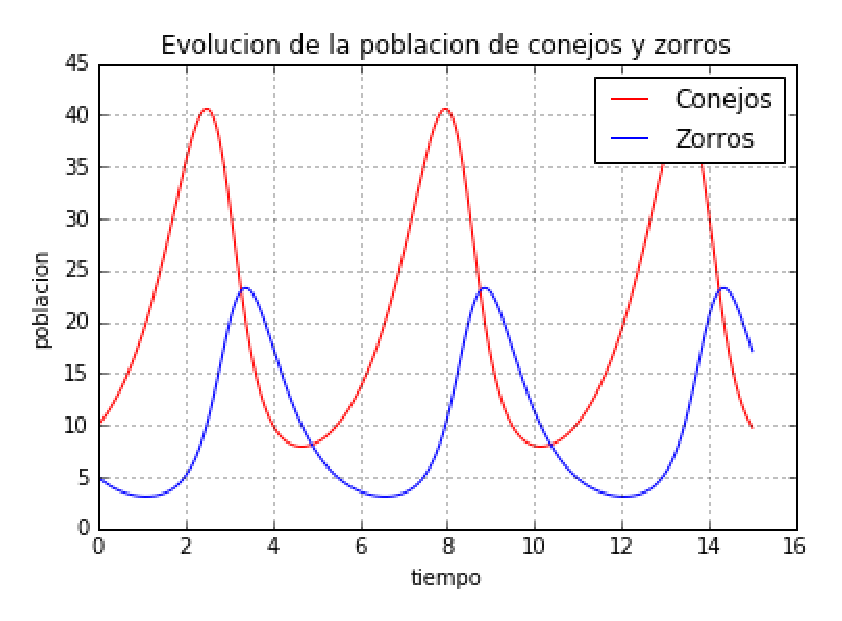
\includegraphics[scale=0.5]{sistemalotka.eps}
\end{figure}
\end{frame}
\begin{frame}
\frametitle{Al considerar un estudio de sistemas dinámicos}
Al darle un giro al abordaje del problema inicial, la información que se obtiene de la evolución de las poblaciones es mayor al utilizar un diagrama de fase.
\\
\begin{figure}
\centering
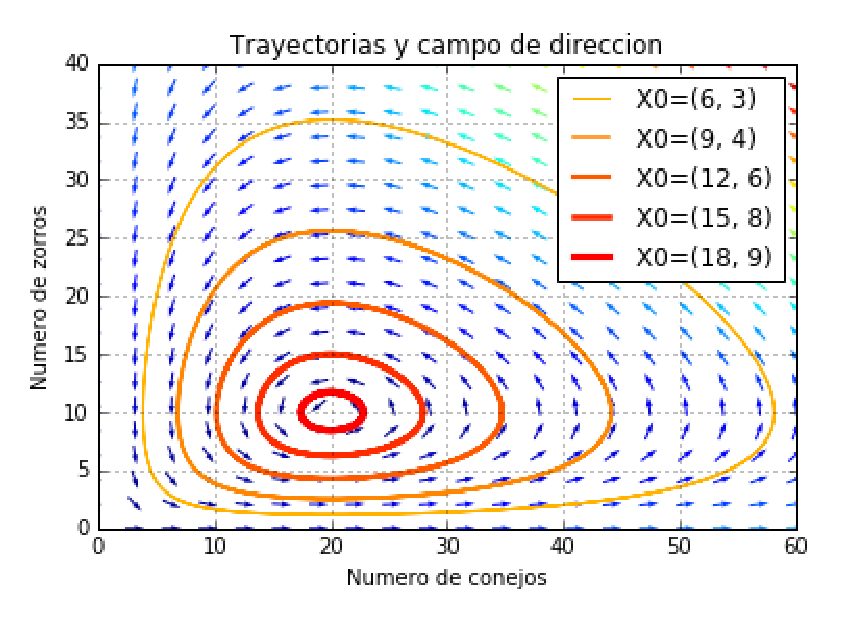
\includegraphics[scale=0.5]{sistemalotkafase.eps}
\end{figure}
\end{frame}
\begin{frame}
\frametitle{La FC en EDP}
La forma más general de una Ecuación Diferencial Parcial (EDP) de segundo orden es
\[ A \dfrac{\partial^{2} U}{\partial x^{2}} + 2B \dfrac{\partial^{2} U}{\partial x \partial y} + C \dfrac{\partial^{2} U}{\partial y^{2}} + D \dfrac{\partial U}{\partial x} + E \dfrac{\partial U}{\partial y} = F \]
Donde $A$, $B$, $C$ y $F$ son funciones arbitrarias de $x$ e $y$.
\end{frame}
\begin{frame}
\frametitle{Un problema clásico: la ecuación de calor.}
La ecuación de calor es:
\[ \dfrac{\partial T(x,t)}{\partial t} = \dfrac{K}{C \rho} \nabla^{2} T(x,t)\]
¿Cómo se resuelve un problema de este tipo?
\\
\medskip
\pause
Con una herramiento del cálculo que se llama ``diferencias finitas'' y con un algoritmo implementado en python.
\end{frame}
\begin{frame}
\frametitle{Solución gráfica}
\begin{figure}
	\centering
	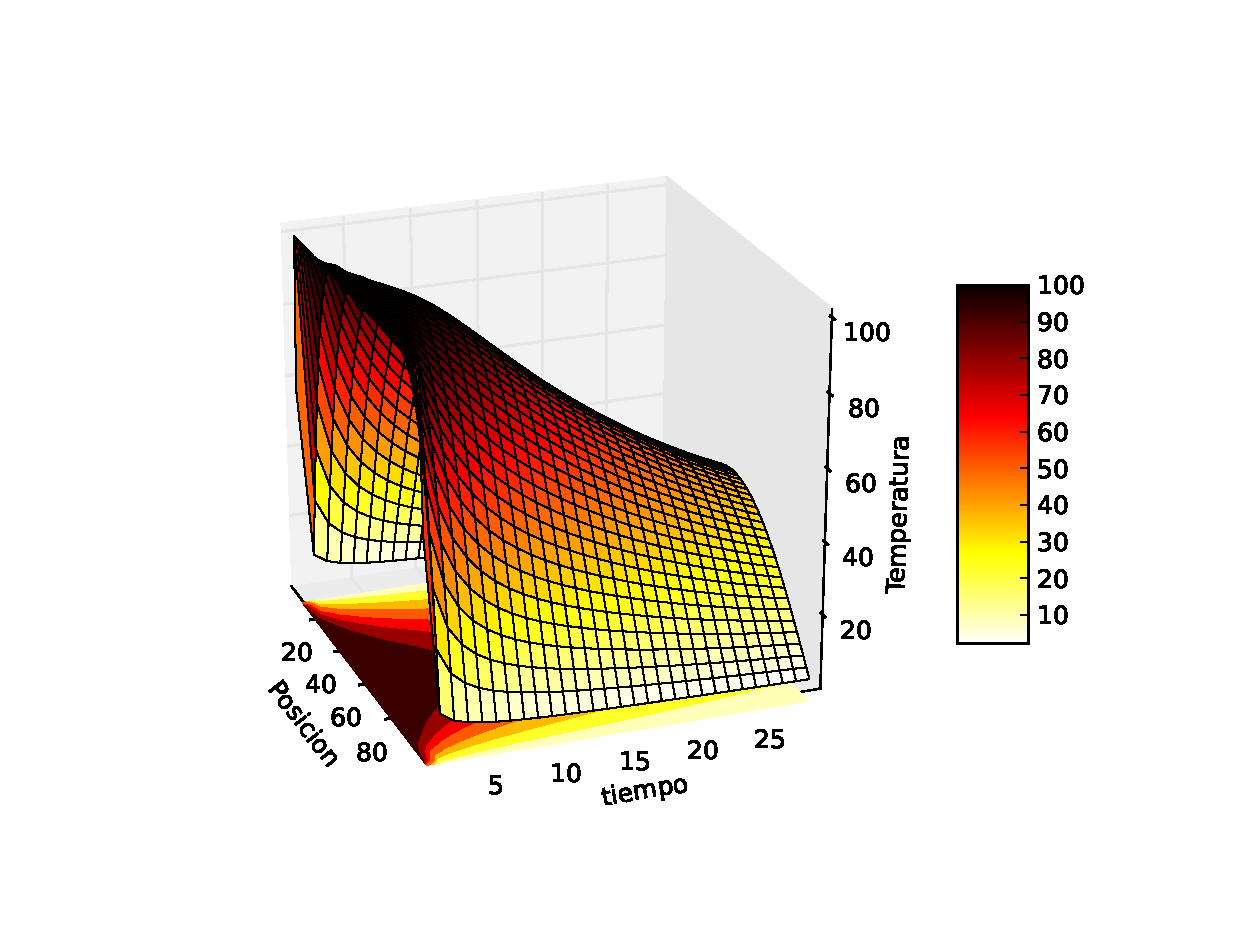
\includegraphics[scale=0.5]{EqCalor01.eps}  
\end{figure}
\end{frame}
\begin{frame}
\frametitle{Es posible modificar los parámetros iniciales.}
\begin{figure}
	\centering
	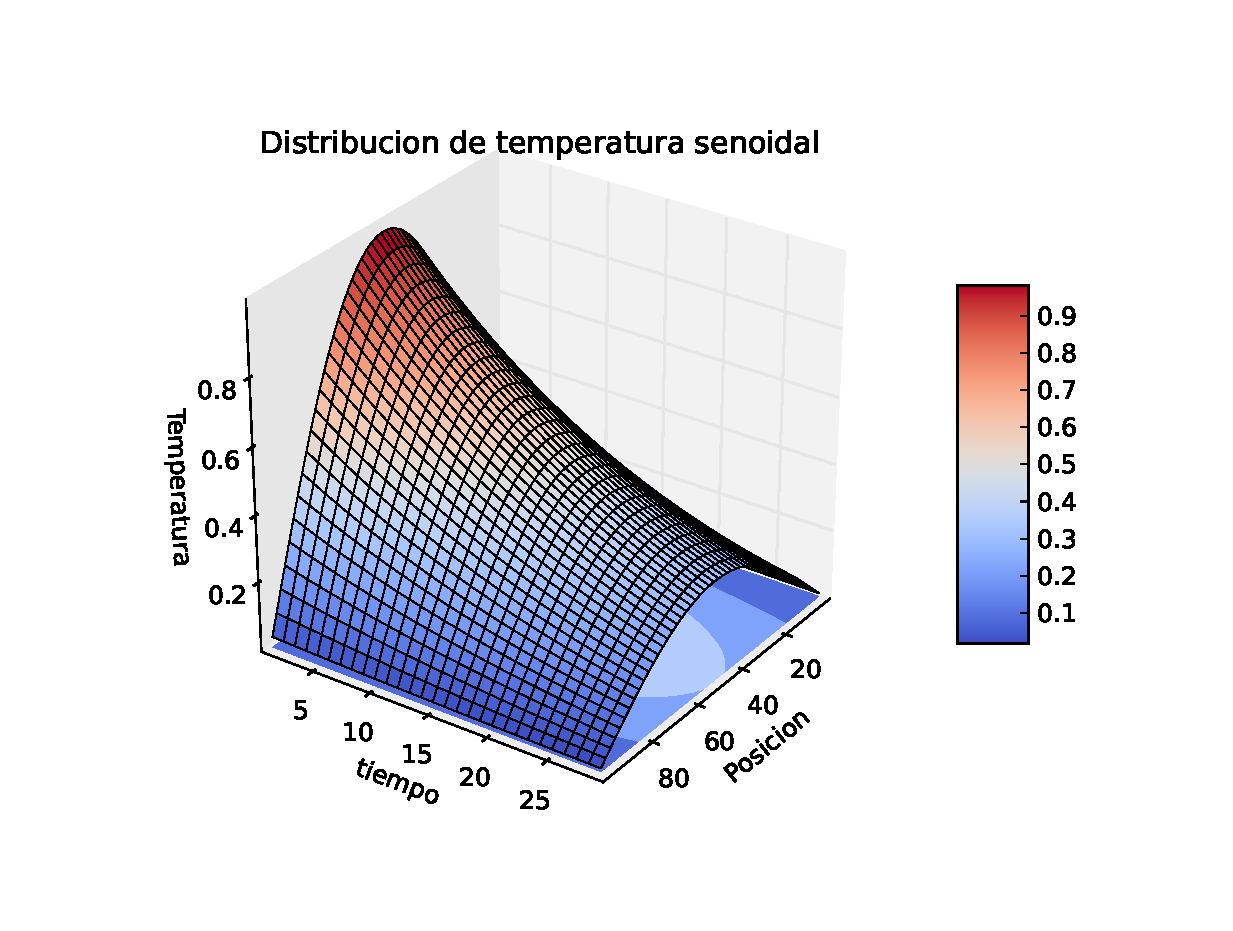
\includegraphics[scale=0.5]{EqCalor04.eps}  
\end{figure}
\end{frame}
\begin{frame}
\begin{figure}
\frametitle{Los cambios no necesariamente son situaciones reales.}
	\centering
	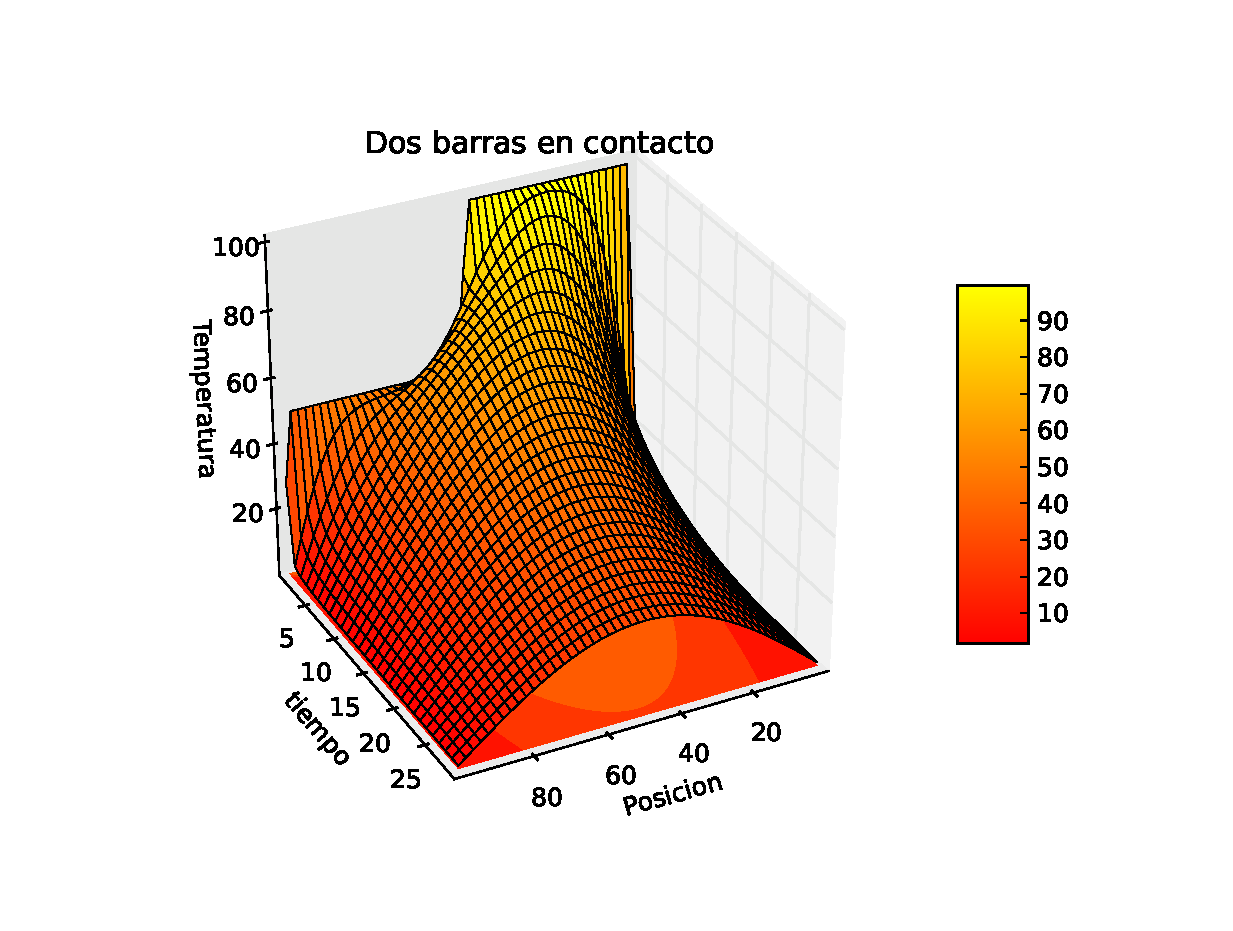
\includegraphics[scale=0.5]{EqCalor06.eps}  
\end{figure}
\end{frame}
\begin{frame}
\frametitle{Es buena idea iniciar con la programación}
Hoy en día es importante y muy necesario contar con habilidades en la programación científica, ya que al lugar donde vayas para comenzar un servicio social, la tesis, un posgrado, se dará por hecho de que sabes manejar algún lenguaje.
\\
\bigskip
Considera que hay lenguajes de fácil aprendizaje, unos tienen ventajas sobre otros, pero la física es siempre la misma, por lo que no importa cuál elijas, lo que cambia es la sintaxis de las instrucciones, pero el algoritmo será básicamente el mismo.
\end{frame}
\begin{frame}
\frametitle{Lo más importante.}
El punto central cuando usamos una computadora para simular un fenómeno físico es: la interpretación que le demos a los resultados.
\\
\medskip
Todo buen físico debe de generar conclusiones a partir de lo que le devuelva un código, recuerda: la física computacional es el medio, no el fin.
\\
\medskip
gus.contreras.m@gmail.com
\end{frame}
\end{document}